% Generated by scripts/make_census_figures.py -- do not edit by hand.
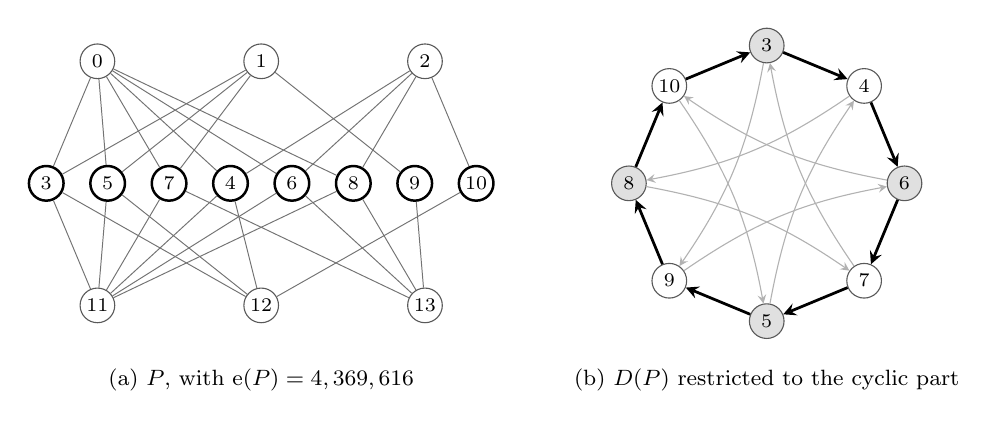
\begin{tikzpicture}[
  x=1cm, y=1cm,
  every node/.style={inner sep=1pt},
  el/.style={circle, draw=black!65, minimum size=4.4mm,
              font=\scriptsize},
  cyc/.style={el, draw=black, line width=0.9pt},
  odd/.style={el, fill=black!12},
  cov/.style={draw=black!55, line width=0.35pt},
  maj/.style={->, >=stealth, draw=black!30, line width=0.4pt},
  hot/.style={->, >=stealth, draw=black, line width=1.0pt},
]
  \node[el] (p11) at (-2.080,0.000) {11};
  \node[el] (p12) at (0.000,0.000) {12};
  \node[el] (p13) at (2.080,0.000) {13};
  \node[cyc] (p3) at (-2.730,1.550) {3};
  \node[cyc] (p5) at (-1.950,1.550) {5};
  \node[cyc] (p7) at (-1.170,1.550) {7};
  \node[cyc] (p4) at (-0.390,1.550) {4};
  \node[cyc] (p6) at (0.390,1.550) {6};
  \node[cyc] (p8) at (1.170,1.550) {8};
  \node[cyc] (p9) at (1.950,1.550) {9};
  \node[cyc] (p10) at (2.730,1.550) {10};
  \node[el] (p0) at (-2.080,3.100) {0};
  \node[el] (p1) at (0.000,3.100) {1};
  \node[el] (p2) at (2.080,3.100) {2};
  \draw[cov] (p3) -- (p0);
  \draw[cov] (p3) -- (p1);
  \draw[cov] (p4) -- (p0);
  \draw[cov] (p4) -- (p2);
  \draw[cov] (p5) -- (p0);
  \draw[cov] (p5) -- (p1);
  \draw[cov] (p6) -- (p0);
  \draw[cov] (p6) -- (p2);
  \draw[cov] (p7) -- (p0);
  \draw[cov] (p7) -- (p1);
  \draw[cov] (p8) -- (p0);
  \draw[cov] (p8) -- (p2);
  \draw[cov] (p9) -- (p1);
  \draw[cov] (p10) -- (p2);
  \draw[cov] (p11) -- (p3);
  \draw[cov] (p11) -- (p4);
  \draw[cov] (p11) -- (p5);
  \draw[cov] (p11) -- (p6);
  \draw[cov] (p11) -- (p7);
  \draw[cov] (p11) -- (p8);
  \draw[cov] (p12) -- (p3);
  \draw[cov] (p12) -- (p4);
  \draw[cov] (p12) -- (p5);
  \draw[cov] (p12) -- (p10);
  \draw[cov] (p13) -- (p6);
  \draw[cov] (p13) -- (p7);
  \draw[cov] (p13) -- (p8);
  \draw[cov] (p13) -- (p9);
  \node[font=\footnotesize] at (0,-0.95) {(a) $P$, with $\mathrm{e}(P)=4,369,616$};
  \node[odd] (m3) at (6.420,3.300) {3};
  \node[el] (m4) at (7.657,2.787) {4};
  \node[odd] (m6) at (8.170,1.550) {6};
  \node[el] (m7) at (7.657,0.313) {7};
  \node[odd] (m5) at (6.420,-0.200) {5};
  \node[el] (m9) at (5.183,0.313) {9};
  \node[odd] (m8) at (4.670,1.550) {8};
  \node[el] (m10) at (5.183,2.787) {10};
  \draw[hot] (m3) to (m4);
  \draw[maj] (m3) to[bend left=12] (m9);
  \draw[hot] (m4) to (m6);
  \draw[maj] (m4) to[bend left=12] (m8);
  \draw[maj] (m5) to[bend left=12] (m4);
  \draw[hot] (m5) to (m9);
  \draw[hot] (m6) to (m7);
  \draw[maj] (m6) to[bend left=12] (m10);
  \draw[maj] (m7) to[bend left=12] (m3);
  \draw[hot] (m7) to (m5);
  \draw[maj] (m8) to[bend left=12] (m7);
  \draw[hot] (m8) to (m10);
  \draw[maj] (m9) to[bend left=12] (m6);
  \draw[hot] (m9) to (m8);
  \draw[hot] (m10) to (m3);
  \draw[maj] (m10) to[bend left=12] (m5);
  \node[font=\footnotesize] at (6.420,-0.95) {(b) $D(P)$ restricted to the cyclic part};
\end{tikzpicture}
